\documentclass{article}
\usepackage{graphicx}
\usepackage{titlesec}
\usepackage{hyperref}
\usepackage{enumitem}
\usepackage{lmodern}
\usepackage{amsmath}
\usepackage{fancyhdr}
\usepackage{textcomp}
\usepackage{lmodern}% http://ctan.org/pkg/lm
\usepackage[table,x11names,svgnames]{xcolor}
\usepackage{soul}
\usepackage{parskip}
\usepackage{multirow}
\usepackage{array}
\usepackage{afterpage}
\usepackage{tabularx}
\usepackage{float}
\usepackage{placeins}
\usepackage{tablefootnote}
\usepackage{microtype}
\usepackage{textcomp}
\usepackage{titlesec}
\usepackage{enumitem}
\usepackage{listings}
\usepackage{subcaption}
\usepackage{verbatim}
\usepackage[htt]{hyphenat}
\usepackage[letterpaper, portrait, margin=1.5in]{geometry}

% Directives
\setlength\extrarowheight{5pt}

\setcounter{secnumdepth}{4}
\titleformat{\paragraph}
{\normalfont\normalsize\bfseries}{\theparagraph}{1em}{}

\begin{document}



\hrulefill \par
{\Large \textbf{Learn to play Go}\par}
{\Large Proposal\par}
\hrulefill \par
\begin{align*}
\mathrm{Albert\ Liu} &&\href{mailto:albertpl@stanford.edu}{albertpl@stanford.edu}\\
\end{align*}

\section{Introduction}
\begin{figure}[H]
\begin{center}
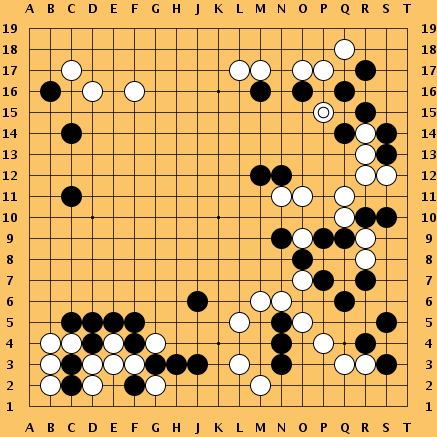
\includegraphics[width=0.25\linewidth]{goboard}
\end{center}
\caption{a snapshot of the Go board}
\label{fig:goboard}
\end{figure}

We formulate Go as a turn-taking, two player, zero-sum game of perfect information. The state space is all possible placements of the stones on the board and the player who plays that turn. The player is either black stone or white stone. The state is fully observable as input. The action space is any legal position a stone can be, given the current state, and a special "pass" action.  The utility for our agent is, 0 for tie, -1 for loss, and +1 for win. We aim to learn to make optimal move to maximum the utility, by observing the board. Figure \ref{fig:goboard} shows a concrete Go board and white stone is making a move at $P15$.

The main challenge is enormous search space, large number of legal move per state, i.e. branching factor, ( $\sim 250$ ) and the difficulty to handcraft a heuristic evaluation function for positions and moves. DeepMind team has made tremendous improvements, particularly AlphaGo \cite{silver2016mastering}, AlphaGoZero \cite{silver2017masteringalphagozero} and AlphaZero \cite{silver2017masteringalphazero} with deep reinforcement learning approaches and self-play.

\section{Evaluation}
Pachi \cite{baudivs2011pachi} is our game engine and we build the simulation environment based on OpenAI's Gym \cite{brockman2016openai} implementation. We plan to have the agent play against the build-in Pachi engine for n trials, which is said to hold KGS 2d rank, and report the average reward.

As for our baseline, we propose two approaches
\begin{enumerate}
  \item
    Random agent, i.e. uniformly choose one of the legal moves.
  \item
    We train a 4-layer convolutional neural network by supervised learning to predict the moves made by expert players. The dataset is from Fox Go Server \cite{FoxGoServer} and contains $9K$ game records of professional players. Following AlphaGoZero, our input feature is a 19x19x17 array, representing 8 boards with each board in two channels, one for current player and the other for opponent. The last channel represents current player.

  We see neither plays good enough against the Pachi engine yet. We need to explore more advanced Reinforcement Learning approaches.
    
\end{enumerate}



\bibliography{reference} 
\bibliographystyle{ieeetr}
\end{document}
